\section{Random Tree Search Algorithm for Finding NE}\label{sec:apx-alg}
We use random tree search algorithm to find the optimum resource allocation in the CSR game.
Each node in the random tree is $n$-dimensional vector denoting an allocation instance.
The search algorithm adds new nodes to the tree by sampling new allocations and optimizing the cost of each allocation iteratively.

The search algorithm starts by randomly generating a few allocation as seeds and stores them in a buffer.
This buffer maintains the highest scoring allocations that we have found so far.
Next, at each iteration, the search algorithm picks an allocation from the buffer.
The algorithm improves the score of the allocation by randomly changing a resource of an unsatisfied player in the allocation. Next, we push back the updated allocation back into the buffer.
By iteratively uptimizing allocations, the search algorithm eventually converges toward the optimal allocation in the game.

%n=number of players
%k=number of resources
%q=size of priority-queue
%p=probabiliy of existence of an edge between two player
% b = size of priority-queue


Figure~\ref{fig:random_tree_1} shows the random tree and the buffer. Each edge between two nodes ${\bf p}_i$ and ${\bf p}_j$ in the random tree denotes the search algorithm found allocation ${\bf p}_j$ by chaning resources of a few players in allocation ${\bf p}_i$. The buffer is a fixed-size priority queue that sorts the allocations according to their score.
Figure~\ref{fig:random_tree_1} shows the progress of search algorithm during one iteration.
At every iteration, we randomly pick an allocation from the buffer, say ${\bf p}_3$. We compute the new allocation ${\bf p}_*$ by changing the resources of the unsatisfied players in allocation ${\bf p}_3$. Next, we compute the radius and saturation of each player in the new allocation ${\bf p}_*$ in order to compute the ${\bf p}_*$'s score. Finally, we insert the new allocation ${\bf p}_*$ into the buffer according to it's score. The buffer is sorted and implemented using a priority queue. If the ${\bf p}_*$ has a better score than the least-scoring allocation in the buffer, in this case ${\bf p}_0$, ${\bf p}_*$ will be pushed to the queue and ${\bf p}_0$ will be evicted. If ${\bf p}_*$ is scoring less than ${\bf p}_*$ we discard the new allocation and continue the search. The algorithm will terminate when we find an allocation that satisfied all players.

\begin{figure}[htb]
\begin{center}
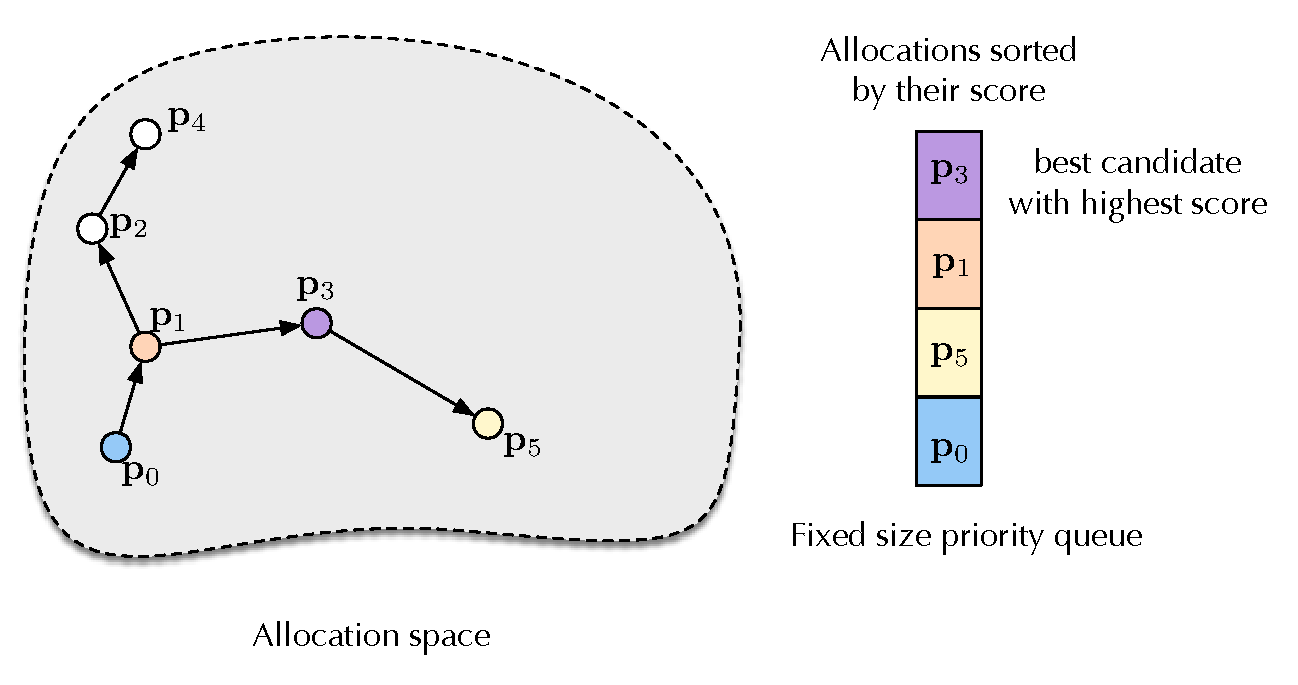
\includegraphics[width=.4\textwidth]{random-tree-figure-1}
\end{center}
\caption{Random tree with 6 sampled allocations ${\bf p}_0\dots {\bf p}_5$. Allocations are sorted in a priority queue of a a fixed size according to their score.}
\label{fig:random_tree_1}
\end{figure}

\begin{figure}[htb]
\begin{center}
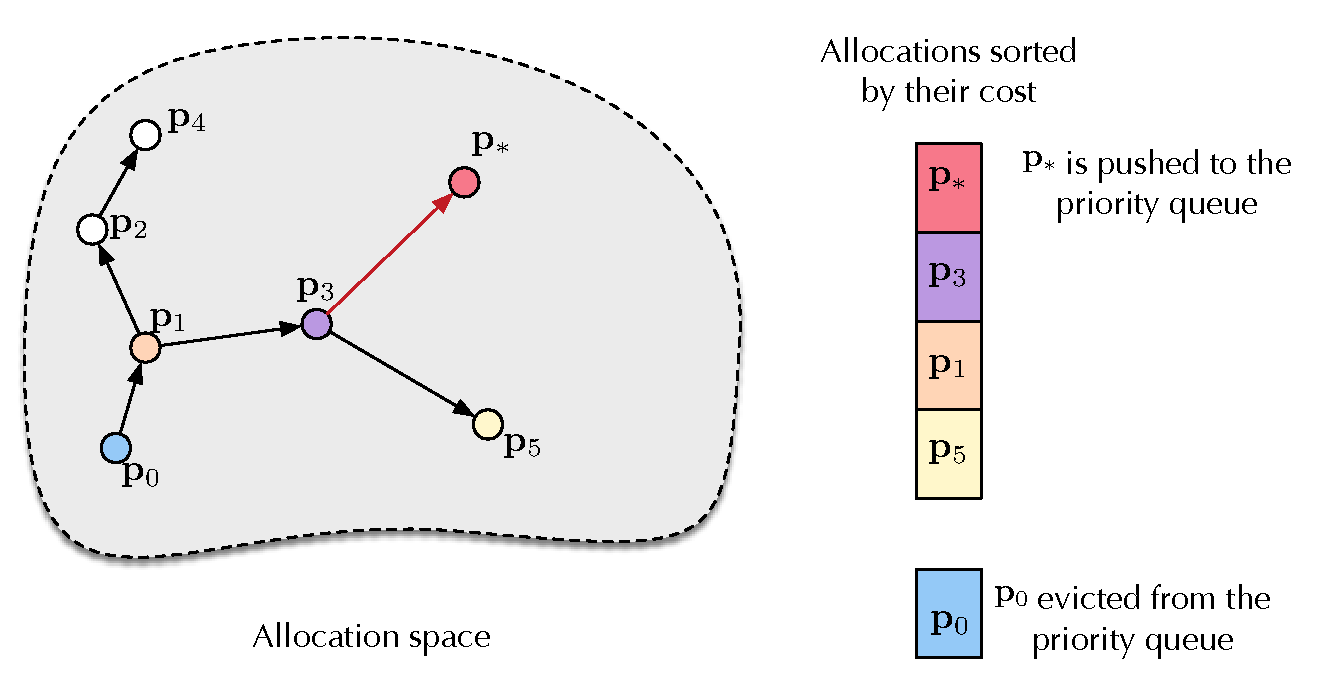
\includegraphics[width=.4\textwidth]{random-tree-figure-2}
\end{center}
\caption{After updating allocation ${\bf p}_3$, we find a new high-scoring allocation ${\bf p}_*$. Pushing ${\bf p}_*$ to the top of the queue evicts the least-scoring allocation ${\bf p}_0$. As a result, we will no longer branch the simulation from ${\bf p}_0$. }
\label{fig:random_tree_2}
\end{figure}

We utilize many heuristics to improve performance of the random tree search algorithm. We will describe these heuristics in more details.

\paragraph{Warmup phase:} Similar to other stochastic search algorithms, the runtime for random tree search depends on the choice of the initial allocation profile. In order to reduce the variance in search, the random tree starts the search by generating multiple randomized allocation as initial seeds. We emprically observed using $n$ (the number of players) iterations in the warmpup phase can substantially reduce overall runtime. In the end of warmpup phase, we sort the seeds according to their score and only keep the $b$ best seeds that we found, where $b$ is the size of the buffer.

\paragraph{Buffer size:} The buffer size $b$ has has a deep impact on how the random tree searches the allocation space. If we choose a very small buffer size, $b=1$, the random tree search becomes a greedy random walk in the space. As a result, the algorithm's performance will degrade and it can get stuck in local minimas. On the other hand,
We emprically observed setting the buffer size at a fixed size 10 yields the optimal performance.

\paragraph{Updating allocations:} At every iteration, we have to make a choice of which player's resource to update in the allocation.
The random tree algorithm updates the resources of a few of unsatisfied players in the allocation.
If we update a very few players, say 1 or 2, the algorithm converges slowly. On the other hand, if we update too many players, specially at the begining, the algorithm is unable to efficiently optimize each allocation. We updates an expected half of the players at each iteration. Furthermore, with a low probability ($5\%$), we will update a player at random (that might even be a satisfied player). These type of intentionally adding error, althought seems counter-intuitive, is shown to be very effective and practical in randomized search algorithms.

%The random tree search algorithm work as follows.
%Initially, we generate a few random allocation as seends and compute the score of each allocation. Then we push these initial seeds into the fixed-size priority queue sorted by each allocation's score. The froniter set is the set of the $n$ highest scoring allocation that we found so far.
%At each iteration, the random tree algorithm pick an allocation from the frontier set, and changes a resource of one of the unsatisfied players. Then the random tree updates the score function and pushes back the new allocation into the frontier set.
%If the new allocation has a better score than the lowest-scoring allocation in the frontier set, we drop the least-score element from the frontier set. As a result, the frontier set always has a fixed-size.

\paragraph{Complexity Analysis:}
In order to understand the computational complexity of the random tree search algorithm, we break-down the computation at every iteration. Each iteration in the random tree search consists of three actions:
i) Picking a node from the frontier set (the priority queue) and changing the allocation,
ii) Updating the raidus and saturation of the new allocation, and
iii) Pushing back the new node back to the priority queue.
The computational complexity of the first part is $O(1)$. The most expensive part of the algorithm is updating the radius and saturation of each player, which requires running a breath-first search in the player graph. The computational complexity of running BFS is $O(n+e)$ where $n$ is the number of the players and $e$ is the number of the edges in the CSR graph. Finally, the computational complexity of inserting the new allocation back to the priority queue is $O(log b)$, where $b$ is the buffer size. Finally, we keep the priority queue sorted in order to make weighted sampling, as a result, the complexity of inserting into the priority queue is $O(b\log^2(b))$. The overal complexity of the algorithm is $O(n\times(n+e)\times b\log^2(b))$.

The random tree search algorithm is probabilistically complete \cite{Lavalle2006}. Therefore, given enought time it will always find the optimal allocation. However, there is no bound on the number of sufficient iterations for finding the optimal allocation. We emprically demonstrate the random tree requires a very few iteration to find the equilibrium points even for very large scale graphs.
